% Grupos e frequências conferidos no inventário outputs/tecnicas-visao-computacional-e-artigos.md.
A síntese dos 26 estudos organiza as técnicas em seis categorias, conforme a
Tabela~\ref{tab:tecnicas-visao-estudos}. As frequências consideram os 17 estudos
com aplicação direta, incluindo componentes descritos nos métodos e comparadores
avaliados. Cada publicação contribui uma vez por grupo, mesmo quando emprega
várias variantes. Os grupos são não exclusivos, de modo que um estudo pode
participar de várias linhas. Os identificadores E01--E26 remetem à autoria e à
referência bibliográfica na Tabela~\ref{tab:estudos-incluidos}.

A preparação reúne operações sobre enquadramento, resolução, intensidade e ruído.
Por exemplo, \citeonline{jitendra2024deep} e \citeonline{jitendra2024heuristic}
descrevem equalização e normalização, \citeonline{nyatte2022} aplicam conversão
para cinza e expansão de gama, e \citeonline{mehta2026} combinam equalização
adaptativa de histograma com limitação de contraste (CLAHE) e filtro bilateral.
O redimensionamento costuma usar $224 \times 224$ pixels, compatível com
redes pré-treinadas no ImageNet \cite{pons2026}.
O aumento abrange transformações geométricas e fotométricas descritas por
\citeonline{baweja2023}, \citeonline{gawali2024}, \citeonline{eita2025} e
\citeonline{jaikishore2021}. Em \citeonline{lima2024skin}, SMOTE produz amostras
no espaço de atributos extraídos pela Inception V3.

As técnicas de localização têm saídas e finalidades distintas. Otsu e morfologia
\cite{nyatte2022}, Fuzzy C-Means com Firefly \cite{jitendra2024heuristic} e
U-Net \cite{jitendra2024deep} delimitam regiões para etapas posteriores.
\citeonline{sanchez2024} avaliam máscaras binárias de ferida e fundo com redes
de segmentação. O detector de \citeonline{eita2025} prediz caixas e classes de
lesões, com supressão não máxima (NMS) das caixas redundantes.

Na extração, os descritores manuais de textura incluem matriz de coocorrência de
níveis de cinza (GLCM), padrões binários locais (LBP), descritor local de Weber
(WLD) e histograma de gradientes orientados (HOG). \citeonline{banerjee2023}
avaliam LBP/WLD e variantes invariantes à rotação em sub-regiões definidas pelo
centro de gravidade. Os dois estudos de Jitendra combinam GLCM e atributos de CNN.
O HSTFC de \citeonline{mehta2026} descreve fusão de LBP/HOG e atributos profundos,
ponderada por atenção, antes de XGBoost. As métricas desse trabalho são agregadas
ao sistema, e a contribuição isolada de HOG ou do classificador fica indeterminada.

A classificação reúne redes profundas e classificadores tradicionais, como os
comparados nas microfotografias histopatológicas de \citeonline{vargasclavijo2025}.
\citeonline{yotsu2023} avaliam ResNet-50 e VGG-16, e \citeonline{beesetty2023}
aprendem similaridade entre pares com poucos exemplos. \citeonline{pons2026}
descrevem classificação em cascata, enquanto a avaliação externa de
\citeonline{deps2026} abrange exclusivamente o segundo estágio da versão beta.
Por isso, a frequência de uso direto da cascata completa é atribuída a E15.
Em \citeonline{jaikishore2021}, a MobileNetV2 foi convertida para
TensorFlow Lite e executada em aplicativo Android em dispositivo periférico.
Em \citeonline{barbieri2022}, a fusão com imagens aparece entre as configurações
testadas. A configuração final selecionada utiliza características clínicas da
lesão e dados do paciente. As arquiteturas e os classificadores específicos estão
detalhados na Subseção~\ref{subsec:rq-modelos-abordagens} e no
Apêndice~\ref{apend:inventario-modelos}.

\begingroup
\small
\setlength{\tabcolsep}{4pt}
\setlength{\parskip}{0pt}
\renewcommand{\arraystretch}{1.12}
\begin{longtable}{|>{\raggedright\arraybackslash}p{3.5cm}|>{\raggedright\arraybackslash}p{6.1cm}|c|>{\raggedright\arraybackslash}p{3.6cm}|}
\caption[Técnicas de visão computacional por estudo]{Grupos de técnicas de visão computacional e estudos com uso direto}\label{tab:tecnicas-visao-estudos}\\ \hline
\textbf{Grupo de técnicas} & \textbf{Variantes e finalidade} & \textbf{n/17} & \textbf{Artigos}\\ \hline
\endfirsthead
\multicolumn{4}{l}{\small\textit{Tabela~\ref{tab:tecnicas-visao-estudos} (continuação)}}\\ \hline
\textbf{Grupo de técnicas} & \textbf{Variantes e finalidade} & \textbf{n/17} & \textbf{Artigos}\\ \hline
\endhead

\multicolumn{4}{r}{\small\textit{continua na próxima página}}\\ 
\endfoot

\endlastfoot
\multicolumn{4}{@{}l}{\textbf{Preparação das imagens}}\\*
\hline
Recorte e centralização & Recorte da ROI, centralização da lesão e ajuste de proporção. E04 usa recorte para desidentificação. & 4/17 & \estudo{E04,E15,E21,E25} \\ \hline
\addlinespace[3pt]
Redimensionamento & Padronização da resolução de entrada, incluindo preenchimento de bordas em E23. & 8/17 & \estudo{E05,E06,E15,E18,E19,E23,E24,E25} \\ \hline
\addlinespace[3pt]
Normalização de intensidades & Reescala de pixels, escore-z ou padronização RGB pelos parâmetros do ImageNet, conforme o estudo. & 7/17 & \estudo{E05,E06,E08,E15,E18,E23,E24} \\ \hline
\addlinespace[3pt]
Conversão para cinza & Conversão RGB para representação em níveis de cinza. & 4/17 & \estudo{E06,E07,E18,E25} \\ \hline
\addlinespace[3pt]
Realce de contraste e iluminação & Equalização de histograma e ajuste adaptativo de contraste em E06/E18, expansão de gama em E07 e CLAHE em E22. & 4/17 & \estudo{E06,E07,E18,E22} \\ \hline
\addlinespace[3pt]
Redução de ruído & Filtro mediano bidimensional em E18 e filtro bilateral adaptativo em E22. & 2/17 & \estudo{E18,E22} \\ \hline
\addlinespace[3pt]
Remoção de pelos & Máscara por limiarização e operações morfológicas descritas no pré-processamento. & 1/17 & \estudo{E23} \\ \hline
\addlinespace[3pt]
\multicolumn{4}{@{}l}{\textbf{Aumento e balanceamento}}\\*
\hline
Transformações geométricas & Rotação, espelhamento, translação, escala, zoom ou recorte aleatório. E06 relata variações de orientação e campo de visão. & 6/17 & \estudo{E06,E14,E19,E23,E24,E25} \\ \hline
\addlinespace[3pt]
Transformações fotométricas & Variações de brilho, saturação, cor, contraste ou exposição. & 2/17 & \estudo{E19,E23} \\ \hline
\addlinespace[3pt]
Desfoque e ruído artificial & Desfoque em E14 e adição de ruído gaussiano em E23. & 2/17 & \estudo{E14,E23} \\ \hline
\addlinespace[3pt]
Aumento sem operações especificadas & E05 menciona aumento de dados. E22 relata Albumentations sem discriminar as transformações. & 2/17 & \estudo{E05,E22} \\ \hline
\addlinespace[3pt]
SMOTE & Geração de amostras sintéticas no espaço de atributos da Inception V3, no conjunto de treino e validação. & 1/17 & \estudo{E26} \\ \hline
\addlinespace[3pt]
\multicolumn{4}{@{}l}{\textbf{Segmentação e detecção}}\\*
\hline
Limiarização e morfologia de lesões & Otsu, dilatação e erosão para delimitar a ROI antes da classificação. & 1/17 & \estudo{E07} \\ \hline
\addlinespace[3pt]
Agrupamento Fuzzy C-Means & FCM com centros otimizados pelo algoritmo do vaga-lume (Firefly), para delimitar a ROI. & 1/17 & \estudo{E18} \\ \hline
\addlinespace[3pt]
Segmentação por redes profundas & U-Net em E06, U-Net/FPN/DeepLabV3 e V3+ em E21, U-Net modificada com atenção a bordas em E22. & 3/17 & \estudo{E06,E21,E22} \\ \hline
\addlinespace[3pt]
Detecção por caixas & YOLOv8n e comparadores YOLOv9t, YOLOv10n, ViT, Faster R-CNN e RetinaNet. & 1/17 & \estudo{E23} \\ \hline
\addlinespace[3pt]
Supressão de caixas redundantes & Supressão não máxima (NMS) durante a inferência do detector. & 1/17 & \estudo{E23} \\ \hline
\addlinespace[3pt]
\multicolumn{4}{@{}l}{\textbf{Extração e combinação de atributos}}\\*
\hline
Descritores de textura & GLCM em E06/E18, estatísticas de textura em E07, LBP/HOG em E22 e LBP/WLD e variantes em E25. & 5/17 & \estudo{E06,E07,E18,E22,E25} \\ \hline
\addlinespace[3pt]
Bordas, forma e dimensão fractal & Canny, Sobel, Gabor e Roberts no fluxo de extração, contornos, zonas homogêneas e dimensão fractal. & 1/17 & \estudo{E07} \\ \hline
\addlinespace[3pt]
Atributos aprendidos por redes profundas & Representações aprendidas por CNNs ou Transformers em classificação, detecção e segmentação, incluindo codificadores e extratores. & 15/17 & \estudo{E04,E05,E06,E13,E14,E15,E17,E18,E19,E21,E22,E23,E24,E25,E26} \\ \hline
\addlinespace[3pt]
Fusão de atributos manuais e profundos & Concatenação de GLCM e CNN em E06/E18, fusão de LBP/HOG e CNN ponderada por atenção no HSTFC de E22. & 3/17 & \estudo{E06,E18,E22} \\ \hline
\addlinespace[3pt]
Fusão de imagens com dados clínicos & Combinações testadas com probabilidades do ramo visual, características clínicas e dados do paciente. & 1/17 & \estudo{E13} \\ \hline
\addlinespace[3pt]
\multicolumn{4}{@{}l}{\textbf{Classificação e aprendizado}}\\*
\hline
Classificação por CNN & Redes convolucionais com saída de classe, incluindo comparadores e a rede siamesa. E04 avalia uma rede existente. & 9/17 & \estudo{E04,E05,E13,E14,E15,E17,E19,E24,E25} \\ \hline
\addlinespace[3pt]
Classificadores tradicionais & SVM/Multi-SVM, BHO-SVM, Random Forest, k-NN/1-NN, árvore, Naive Bayes, ANN convencional, regressão logística ou XGBoost. & 9/17 & \estudo{E06,E07,E08,E13,E17,E18,E22,E25,E26} \\ \hline
\addlinespace[3pt]
Transferência de aprendizado & Ajuste de redes pré-treinadas, congelamento de camadas ou reutilização de representações como extratoras. & 7/17 & \estudo{E05,E13,E17,E19,E21,E24,E26} \\ \hline
\addlinespace[3pt]
Classificação em cascata & Triagem inicial seguida de classificação entre 12 DTNs cutâneas. E15 documenta o uso dos dois estágios. & 1/17 & \estudo{E15} \\ \hline
\addlinespace[3pt]
Similaridade com poucos exemplos & Rede siamesa, pares de imagens, distância L2 e perda contrastiva em tarefas n-way k-shot. & 1/17 & \estudo{E17} \\ \hline
\addlinespace[3pt]
\multicolumn{4}{@{}l}{\textbf{Explicabilidade visual}}\\*
\hline
Visualização de ativações & Visualização das ativações das camadas convolucionais da LeprosyNet e dos comparadores. & 1/17 & \estudo{E14} \\ \hline
\addlinespace[3pt]
Sensibilidade à oclusão & Mapas do efeito de ocultar regiões da imagem sobre a predição. & 1/17 & \estudo{E14} \\ \hline
\addlinespace[3pt]
Grad-CAM & Mapas de ativação de classe ponderados por gradientes. & 1/17 & \estudo{E14} \\ \hline
\addlinespace[3pt]
Saliência por gradientes da entrada & Gradientes de classificação e localização em relação aos pixels da entrada do YOLOv8n. & 1/17 & \estudo{E23} \\ \hline
\addlinespace[3pt]
\end{longtable}
\fonte{Autores, a partir dos 17 estudos com aplicação direta. Grupos não exclusivos.}
\endgroup

As Figuras~\ref{fig:tecnicas-preparacao-aumento},
\ref{fig:tecnicas-segmentacao-atributos} e
\ref{fig:tecnicas-classificacao-xai} apresentam até cinco grupos por categoria,
selecionados pela frequência decrescente e, nos empates, pela ordem alfabética.
As barras indicam publicações com uso documentado. Os grupos completos e seus
artigos estão na Tabela~\ref{tab:tecnicas-visao-estudos}.

\clearpage
\begin{figure}[p]
\centering
\caption{Frequência dos grupos de técnicas: preparação das imagens e aumento de dados}
\label{fig:tecnicas-preparacao-aumento}
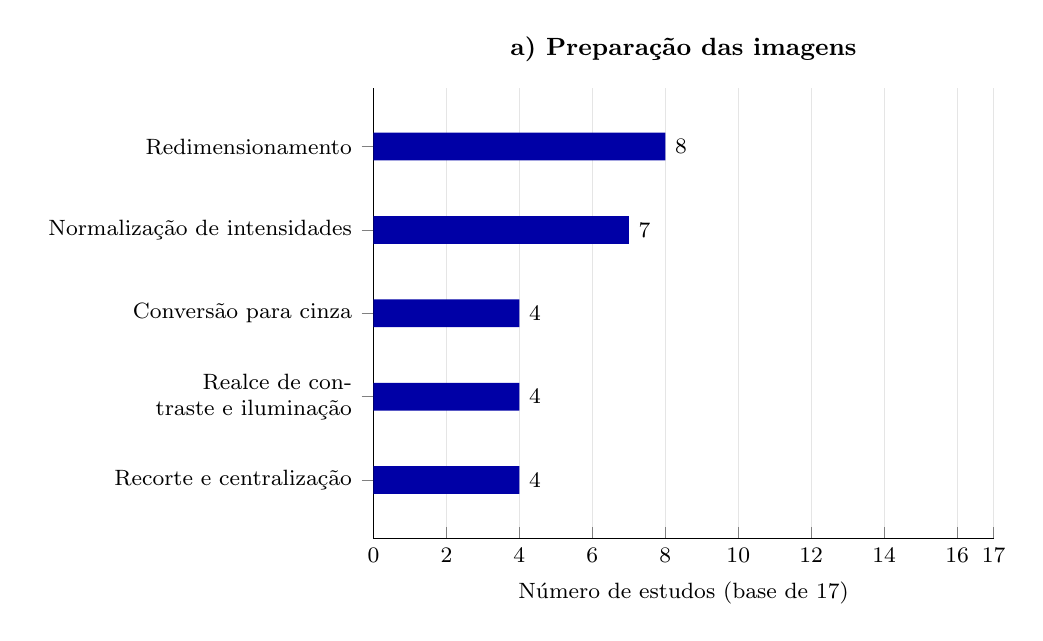
\begin{tikzpicture}
\begin{axis}[
width=0.78\textwidth, height=7.3cm,
xbar, bar width=10pt, xmin=0, xmax=17,
xtick={0,2,4,6,8,10,12,14,16,17},
xlabel={Número de estudos (base de 17)},
ymin=-0.7, ymax=4.7,
y dir=reverse, ytick={0,1,2,3,4},
yticklabels={{Redimensionamento},{Normalização de intensidades},{Conversão para cinza},{Realce de contraste e iluminação},{Recorte e centralização}},
yticklabel style={font=\footnotesize, text width=4.0cm, align=right},
xticklabel style={font=\footnotesize},
label style={font=\footnotesize},
title={a) Preparação das imagens},
title style={font=\small\bfseries},
axis x line*=bottom, axis y line*=left,
xmajorgrids=true, grid style={gray!20},
point meta=x, nodes near coords,
every node near coord/.append style={font=\footnotesize,anchor=west},
]
\addplot[fill=blue!65!black, draw=none] coordinates {
(8,0)
(7,1)
(4,2)
(4,3)
(4,4)
};
\end{axis}
\end{tikzpicture}
\par\vspace{0.8cm}
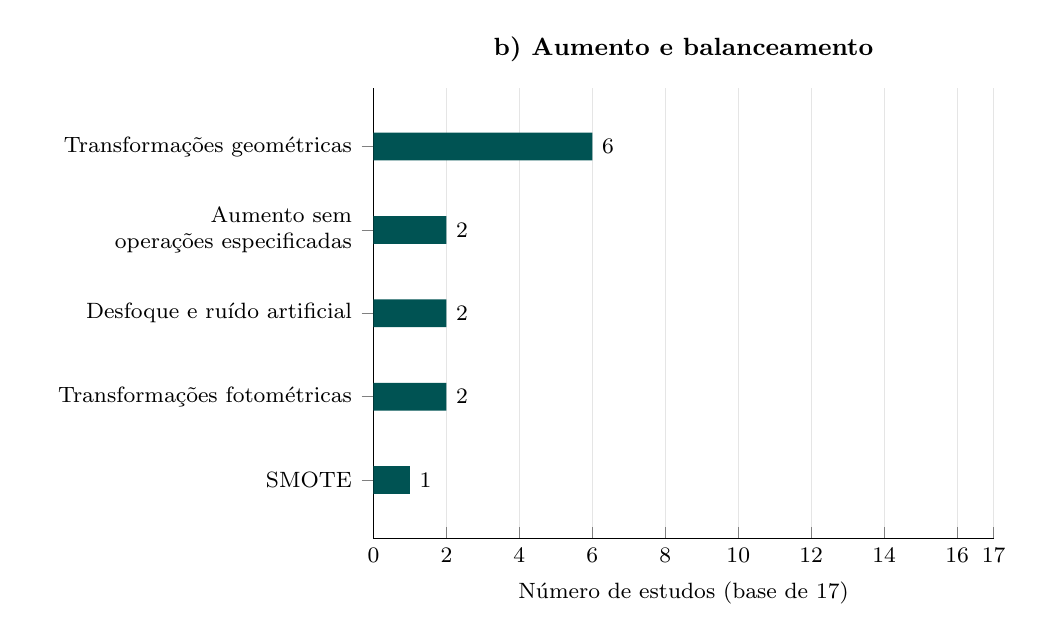
\begin{tikzpicture}
\begin{axis}[
width=0.78\textwidth, height=7.3cm,
xbar, bar width=10pt, xmin=0, xmax=17,
xtick={0,2,4,6,8,10,12,14,16,17},
xlabel={Número de estudos (base de 17)},
ymin=-0.7, ymax=4.7,
y dir=reverse, ytick={0,1,2,3,4},
yticklabels={{Transformações geométricas},{Aumento sem operações especificadas},{Desfoque e ruído artificial},{Transformações fotométricas},{SMOTE}},
yticklabel style={font=\footnotesize, text width=4.0cm, align=right},
xticklabel style={font=\footnotesize},
label style={font=\footnotesize},
title={b) Aumento e balanceamento},
title style={font=\small\bfseries},
axis x line*=bottom, axis y line*=left,
xmajorgrids=true, grid style={gray!20},
point meta=x, nodes near coords,
every node near coord/.append style={font=\footnotesize,anchor=west},
]
\addplot[fill=teal!65!black, draw=none] coordinates {
(6,0)
(2,1)
(2,2)
(2,3)
(1,4)
};
\end{axis}
\end{tikzpicture}
\fonte{Autores, a partir dos 17 estudos com aplicação direta. Grupos não exclusivos, com uma ocorrência por estudo em cada grupo.}
\end{figure}

\begin{figure}[p]
\centering
\caption{Frequência dos grupos de técnicas: segmentação, detecção e extração de atributos}
\label{fig:tecnicas-segmentacao-atributos}
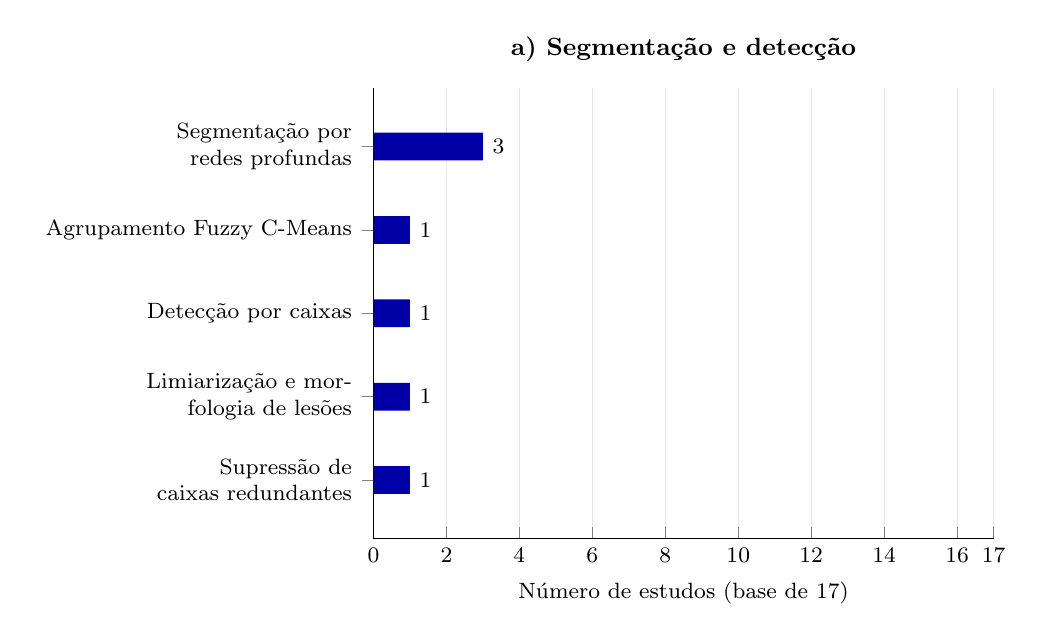
\begin{tikzpicture}
\begin{axis}[
width=0.78\textwidth, height=7.3cm,
xbar, bar width=10pt, xmin=0, xmax=17,
xtick={0,2,4,6,8,10,12,14,16,17},
xlabel={Número de estudos (base de 17)},
ymin=-0.7, ymax=4.7,
y dir=reverse, ytick={0,1,2,3,4},
yticklabels={{Segmentação por redes profundas},{Agrupamento Fuzzy C-Means},{Detecção por caixas},{Limiarização e morfologia de lesões},{Supressão de caixas redundantes}},
yticklabel style={font=\footnotesize, text width=4.0cm, align=right},
xticklabel style={font=\footnotesize},
label style={font=\footnotesize},
title={a) Segmentação e detecção},
title style={font=\small\bfseries},
axis x line*=bottom, axis y line*=left,
xmajorgrids=true, grid style={gray!20},
point meta=x, nodes near coords,
every node near coord/.append style={font=\footnotesize,anchor=west},
]
\addplot[fill=blue!65!black, draw=none] coordinates {
(3,0)
(1,1)
(1,2)
(1,3)
(1,4)
};
\end{axis}
\end{tikzpicture}
\par\vspace{0.8cm}
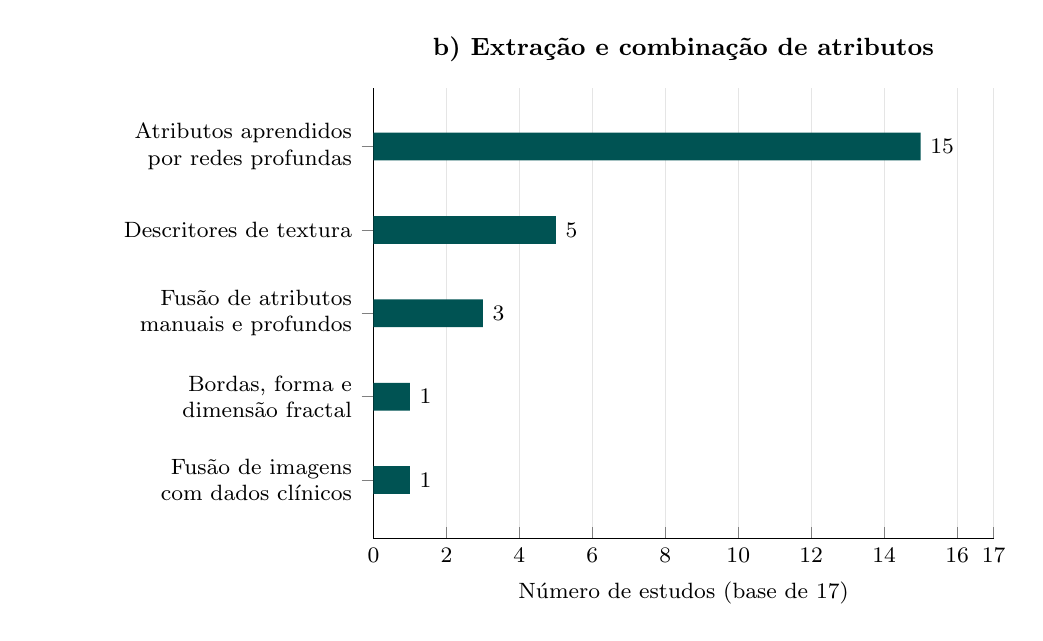
\begin{tikzpicture}
\begin{axis}[
width=0.78\textwidth, height=7.3cm,
xbar, bar width=10pt, xmin=0, xmax=17,
xtick={0,2,4,6,8,10,12,14,16,17},
xlabel={Número de estudos (base de 17)},
ymin=-0.7, ymax=4.7,
y dir=reverse, ytick={0,1,2,3,4},
yticklabels={{Atributos aprendidos por redes profundas},{Descritores de textura},{Fusão de atributos manuais e profundos},{Bordas, forma e dimensão fractal},{Fusão de imagens com dados clínicos}},
yticklabel style={font=\footnotesize, text width=4.0cm, align=right},
xticklabel style={font=\footnotesize},
label style={font=\footnotesize},
title={b) Extração e combinação de atributos},
title style={font=\small\bfseries},
axis x line*=bottom, axis y line*=left,
xmajorgrids=true, grid style={gray!20},
point meta=x, nodes near coords,
every node near coord/.append style={font=\footnotesize,anchor=west},
]
\addplot[fill=teal!65!black, draw=none] coordinates {
(15,0)
(5,1)
(3,2)
(1,3)
(1,4)
};
\end{axis}
\end{tikzpicture}
\fonte{Autores, a partir dos 17 estudos com aplicação direta. Grupos não exclusivos, com uma ocorrência por estudo em cada grupo.}
\end{figure}

\begin{figure}[p]
\centering
\caption{Frequência dos grupos de técnicas: classificação, aprendizado e explicabilidade visual}
\label{fig:tecnicas-classificacao-xai}
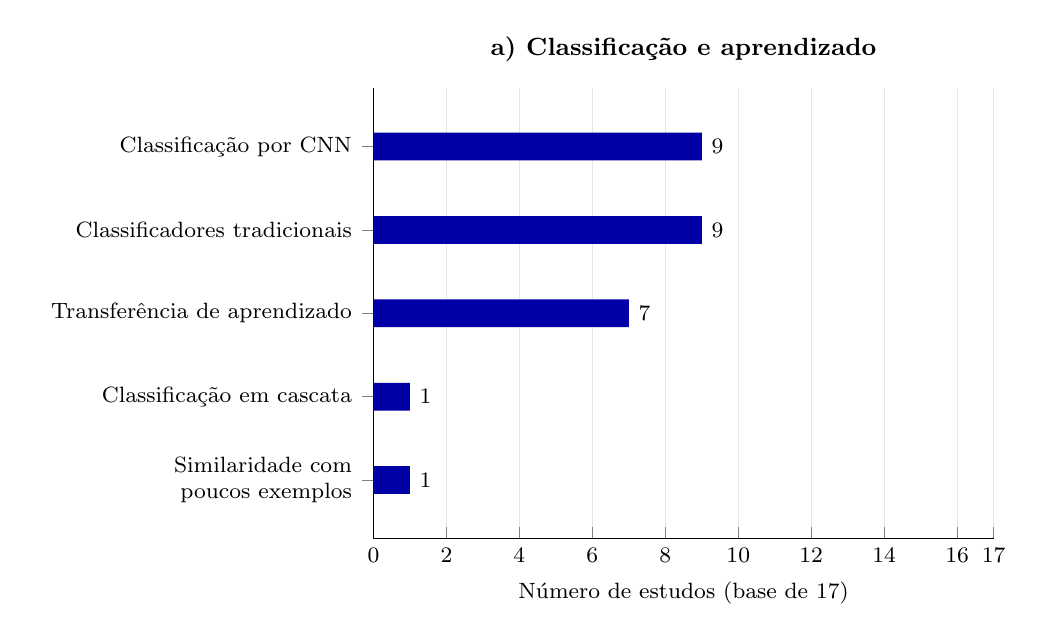
\begin{tikzpicture}
\begin{axis}[
width=0.78\textwidth, height=7.3cm,
xbar, bar width=10pt, xmin=0, xmax=17,
xtick={0,2,4,6,8,10,12,14,16,17},
xlabel={Número de estudos (base de 17)},
ymin=-0.7, ymax=4.7,
y dir=reverse, ytick={0,1,2,3,4},
yticklabels={{Classificação por CNN},{Classificadores tradicionais},{Transferência de aprendizado},{Classificação em cascata},{Similaridade com poucos exemplos}},
yticklabel style={font=\footnotesize, text width=4.0cm, align=right},
xticklabel style={font=\footnotesize},
label style={font=\footnotesize},
title={a) Classificação e aprendizado},
title style={font=\small\bfseries},
axis x line*=bottom, axis y line*=left,
xmajorgrids=true, grid style={gray!20},
point meta=x, nodes near coords,
every node near coord/.append style={font=\footnotesize,anchor=west},
]
\addplot[fill=blue!65!black, draw=none] coordinates {
(9,0)
(9,1)
(7,2)
(1,3)
(1,4)
};
\end{axis}
\end{tikzpicture}
\par\vspace{0.8cm}
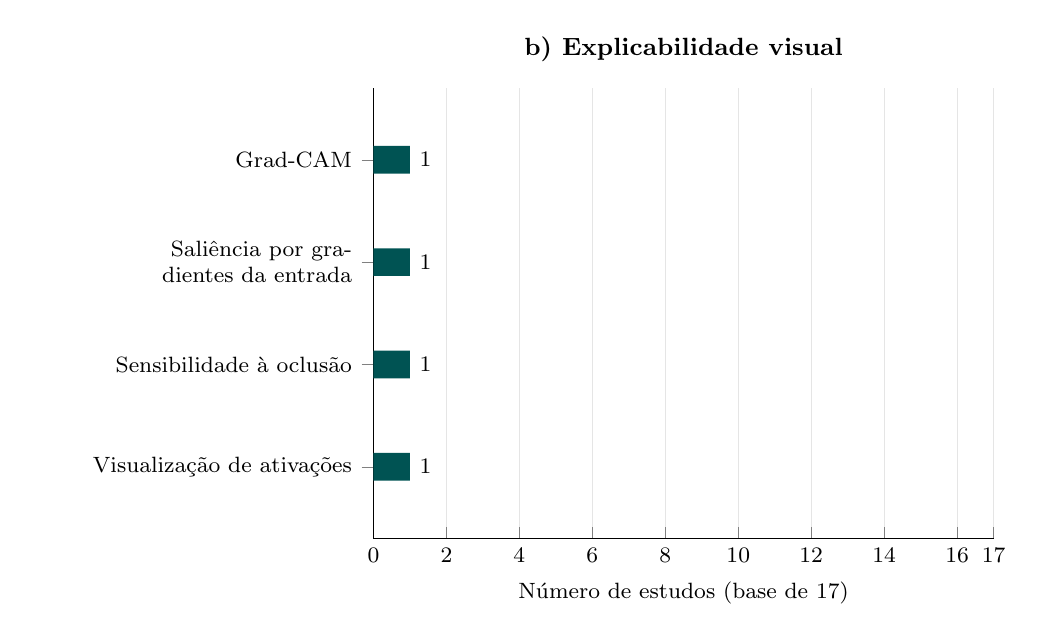
\begin{tikzpicture}
\begin{axis}[
width=0.78\textwidth, height=7.3cm,
xbar, bar width=10pt, xmin=0, xmax=17,
xtick={0,2,4,6,8,10,12,14,16,17},
xlabel={Número de estudos (base de 17)},
ymin=-0.7, ymax=3.7,
y dir=reverse, ytick={0,1,2,3},
yticklabels={{Grad-CAM},{Saliência por gradientes da entrada},{Sensibilidade à oclusão},{Visualização de ativações}},
yticklabel style={font=\footnotesize, text width=4.0cm, align=right},
xticklabel style={font=\footnotesize},
label style={font=\footnotesize},
title={b) Explicabilidade visual},
title style={font=\small\bfseries},
axis x line*=bottom, axis y line*=left,
xmajorgrids=true, grid style={gray!20},
point meta=x, nodes near coords,
every node near coord/.append style={font=\footnotesize,anchor=west},
]
\addplot[fill=teal!65!black, draw=none] coordinates {
(1,0)
(1,1)
(1,2)
(1,3)
};
\end{axis}
\end{tikzpicture}
\fonte{Autores, a partir dos 17 estudos com aplicação direta. Grupos não exclusivos, com uma ocorrência por estudo em cada grupo.}
\end{figure}

\clearpage
Na explicabilidade, \citeonline{baweja2023} apresentam visualização de ativações,
sensibilidade à oclusão e Grad-CAM, e \citeonline{eita2025} geram saliência por
gradientes das saídas em relação à imagem de entrada. Esses mapas permitem
examinar regiões associadas às predições, cuja pertinência clínica requer
avaliação própria.

Como operações auxiliares, \citeonline{yotsu2023} usam análise de componentes
principais (PCA) para projetar atributos em duas dimensões e examinar as
representações. \citeonline{beesetty2023} usam agrupamento de Ward sobre atributos
morfológicos anotados para formar subclasses. \citeonline{sanchez2024} descrevem
anotação manual de máscaras e caixas no CVAT, e \citeonline{barbieri2022} usam
VGG Image Annotator na anotação. \citeonline{pons2026} realizam deduplicação por
similaridade visual profunda antes do particionamento, e \citeonline{sanchez2024}
relatam remoção de duplicatas na curadoria. O mascaramento seletivo em
\citeonline{deps2026} serve à desidentificação.

As revisões de \citeonline{fernandes2024} e \citeonline{andrade2025} sintetizam
estudos com descritores, redes profundas e geração de imagens por GAN, incluindo
a variante WGAN-GP reportada por Fernandes. A comparação de DCT e DFT em
\citeonline{banerjee2023} remete a resultados de trabalho anterior. Essas menções
são evidências secundárias na presente síntese. As revisões de
\citeonline{goswami2026} e \citeonline{ahikpa2025} retomam classificação por imagens,
few-shot e combinações de atributos de estudos primários. \citeonline{prayitno2026}
incluem o AI4Leprosy entre aplicações de saúde digital, e
\citeonline{innocent2026} discutem saliência, Grad-CAM e atenção na literatura.
\citeonline{deps2024} apresentam uma perspectiva sobre análise visual e apoio
clínico. \citeonline{yotsu2025} discutem imagens multiespectrais e térmicas como
possibilidades. O protocolo de \citeonline{sall2025} descreve a avaliação planejada
do aplicativo da OMS. Essas nove publicações contribuem para a síntese narrativa,
e as frequências são atribuídas aos estudos que aplicaram diretamente as técnicas.

